\documentclass[11pt,a4paper]{report}

\usepackage{microtype}
\usepackage[utf8]{inputenc}
\usepackage{float}
\usepackage{graphicx}
\graphicspath{{./images/}}
\usepackage[left=1.00cm, right=1.00cm, top=1.00cm, bottom=2.00cm]{geometry}
\author{Stéphane FEUGA\\{\small sfeuga@member.fsf.org}}
\title{{\Huge Dossier de synthèse de pratique professionnel\\
Titre Développeur Logiciel}\\
{\normalsize Stage du 02/04/2014 au 31/05/2014 pour l'association Uncanny}}
\date {En date du 02/06/2014}
\begin{document}

\maketitle

\vspace*{\stretch{1}}
\begin{center}
This page intentionally left blank
\footnotetext{Ce document est rédigé en \LaTeX - l'intégralité de ce projet à été réalisé avec des outils sous licence libre}
\thispagestyle{empty}
\end{center}
\vspace*{\stretch{1}}

\tableofcontents

\chapter{Présentation}
	\section{Introduction}
		\paragraph*{}
	\section{Historique}
		\paragraph*{}
	\section{L'Association Uncanny}
		\paragraph*{}
	\section{Compétences à mettre en œuvre}
		\paragraph*{\indent Compétence Obligatoire :} Développer une interface utilisateur (page 19 du REAC et page 8 du RC).
		\paragraph*{\indent Compétence Choisie :} Mettre en œuvre une solution de gestion de contenu ou d’e-commerce (page 22 du REAC et page 8 ru RC).
	\section{Remerciements}
		\paragraph*{}Tout d'abord, je souhaite  remercier Mr Cédric CHERDEL et Mr Laurent CEBE de l'association Uncanny qui m'ont offert la possibilité d'avoir un sujet de stage en adéquation avec mes capacités et les compétences à mettre en œuvre pour la validation de ce stage.
		\paragraph*{}Je souhaite aussi remercier Gabriel BLOCK, Emanuelle FERRAND, Erwan FOURNEL et Florence \linebreak NATIVELLE, de l'I.M.I.E., pour leurs implications dans cette formation.
		\paragraph*{}Je souhaite enfin remercier Ada Lovelace\footnote{https://fr.wikipedia.org/wiki/Ada\_Lovelace} sans qui nous ne serions pas là.

\chapter{Mission}
	\section{Présentation du projet}
		Le projet est la mise en place de deux sites internet pour promouvoir les projets et activités de l'association Uncanny et plus particulièrement de Cédric Cherdel. 
		\subsection{Objectifs}
			\begin{enumerate}
				\item Une page d'accueil animé donnant accès aux contenus.\\
				Cette page sera en HTML5 et animé avec CSS3 et jQuery.
				\item Création d'un thème en HTML5 pour un CMS.
				\item Un site internet sur la production de danse contemporaine.\\
				Mise en place du CMS.
				\item Un site lié à l'activité de massage THAÏ de Cédric.\\
				Mise en place du CMS.
			\end{enumerate}
		\subsection{Cible}
			\begin{itemize}
				\item Les professionnels de la Danse
				\item Les particuliers
				\item Les compagnies de Danse
				\item Les Mairies
				\item Les Départements et Régions
			\end{itemize}
		\subsection{Les acteurs}
			\begin{itemize}
				\item Cédric CHERDEL
				\item Laurent CEBE
				\item Stéphane FEUGA
			\end{itemize}
		\subsection{L'existant}
			\begin{itemize}
				\item Une charte Graphique (pas fini au début du projet)
				\item Une liste de contact pour la newsletter
				\item Des documentations sur les projets de danse
			\end{itemize}
	\section{Fonctionnalités \& Contraintes}
		\paragraph*{}En tout premier lieu, j'ai aidé par un questionnaire de question simples (pour qui, pour quoi, comment, avec quoi...) à définir les principales fonctionnalités ainsi que les contraintes liées.
		\paragraph*{}La scission en deux site distinct, à été rapidement abordé car dans l'avenir, l'activité de Massage sera indépendante de l'association pour des raisons fiscales. J'ai donc proposé plusieurs options de réalisation par site, à savoir de simples" sites en HTML, la mise en place de Wordpress\footnote{http://wordpress.org/}, ou encore l'utilisation du CMS JekyllRB\footnote{http://jekyllrb.com/} qui à la particularité d'être très flexible, d'utiliser le Markdown\footnote{http://daringfireball.net/projects/markdown/} pour la rédaction des articles et de ne pas avoir besoin de moteur de base de donné pour fonctionner.
		\paragraph*{}Dans un premier temps, j'ai proposé la solution déjà éprouvé de Wordpress pour la réalisation des premier tests. J'ai donc commencé par définir les actions des différents acteurs (voir la modélisation UML plus loin dans ce rapport). Puis j'ai proposé l'utilisation de licence GNU pour l'intégralité du projet ce qui à été très favorablement accepté, nous avons aussi défini le périmètre des applications (Sites Web).
		\paragraph*{}Lors de ma présentation des avantages et inconvénients des licences libres et plus particulièrement les licences\footnote{http://www.gnu.org/licenses/licenses.html} GNU/GPL v3, GNU/LGPL v3, GNU/AGPL v3 et GNU FDL v1.3, j'ai indiqué qu'une bonne pratique serai d'utilisé des outils de production libres, notre choix c'est donc porté sur Inkscape\footnote{http://www.inkscape.org/fr/}, GIMP\footnote{http://www.gimp.org/}, Vim\footnote{http://www.vim.org/} ainsi \LaTeX \footnote{http://www.latex-project.org/}. L'utilisation de systèmes d'exploitation libre à aussi été retenu, lors de ce développement, nous utiliserons Fedora ainsi que Debian pour le serveur de production.\\
		L'utilisation de ces licences est tout à fait dans l'esprit de partage que l'on retrouve dans les spectacles de danse contemporaine, c'est dans cette logique qu'à été créer l'association Uncanny.
		\paragraph*{}Une des principales contrainte était d'avoir un système simple à modifié tans sur le contenu que sur le plan graphique. Au autre contrainte est d'avoir un système très simple à sauvegarder et a remettre en œuvre lors de pannes ou de mauvaises utilisations. La réalisation de site web en HTML pur à donc été écarté car la complexité requise lors de modification ne correspond pas aux attentes du client.
		\paragraph*{}Dans un second temps, j'ai réalisé deux présentations, la première sur Wordpress et l'autre sur JekyllRB.
		Wordpress à l'avantage d'être très simple à modifier pour peux que l'on souhaite se basé sur un thème existant, le nombre de greffons disponibles est aussi l'assurance de réaliser divers fonctions très simplement.
		\paragraph*{}JekyllRB à quand à lui l'avantage de produire des sites statiques sans besoin de base de donnée. Les sites produits sont plus rapide à chargé qu'un site sous Wordpress. L'autre avantage est que sa modification graphique ce fait uniquement des fichiers plats (fichier CSS et fichier HTML ou Markdown). ils ne nécessite que peux de compétences (du CSS, et peu d'HTML, des duplication de fichiers et de l'huile de coude). Enfin la sauvegarde de l'intégralité du site se fait par une simple copie de dossier, tout étant des fichiers (pas de moteur de base de donnée). La production de nouveau articles ou description de projet se fait soir en HTML ou en Markdown.
		\paragraph*{}Lors de la validation du périmètre de l'application et du cahier des charges, JekyllRB à été retenu pour ces projets avec une possibilité de passage à Wordpress si le nombre d'article augmente fortement.
		\newpage

	\section{L'Expérience Utilisateur et l'Accessibilité}
		\subsection{Le Maquettage}
			\paragraph*{Zoning}Les premiers éléments que j'ai réalisé ont été les zoning des deux sites. J'ai volontairement choisi d'utiliser un minimum de zone afin de simplifier la navigation de façon à favoriser l'expérience utilisateur. Ces éléments ont été validé par le graphiste (Laurent).
				\begin{figure}[H]
					\centering
					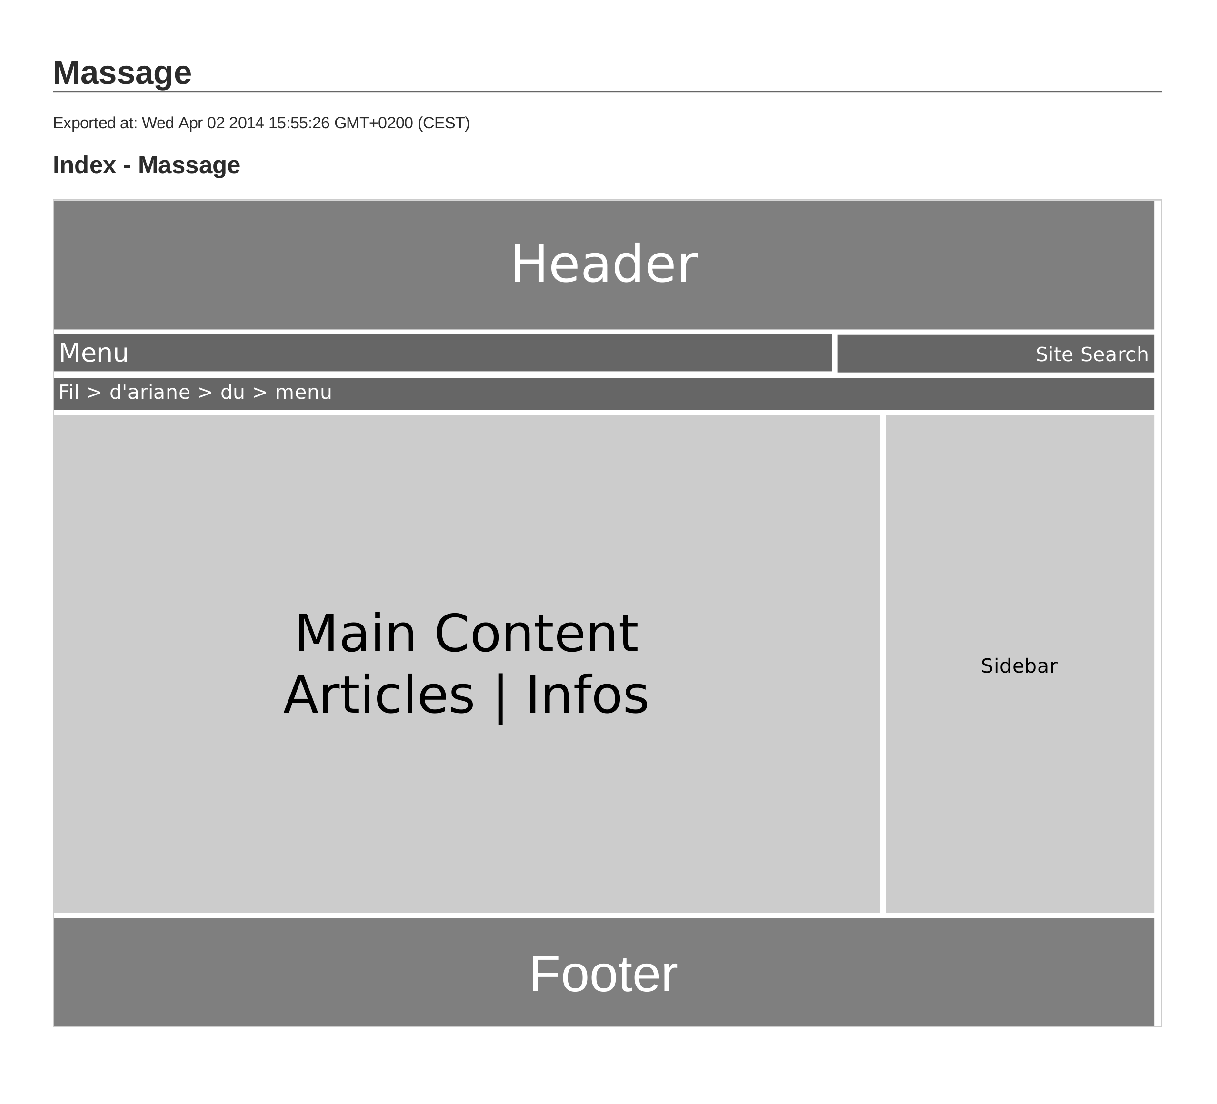
\includegraphics[height=10cm]{Zone-Massage.eps}
					\caption{Exemple de Zoning pour le site "Massage"}
					\label{fig:Zoning Massage}
				\end{figure}
				\begin{figure}[H]
					\centering
					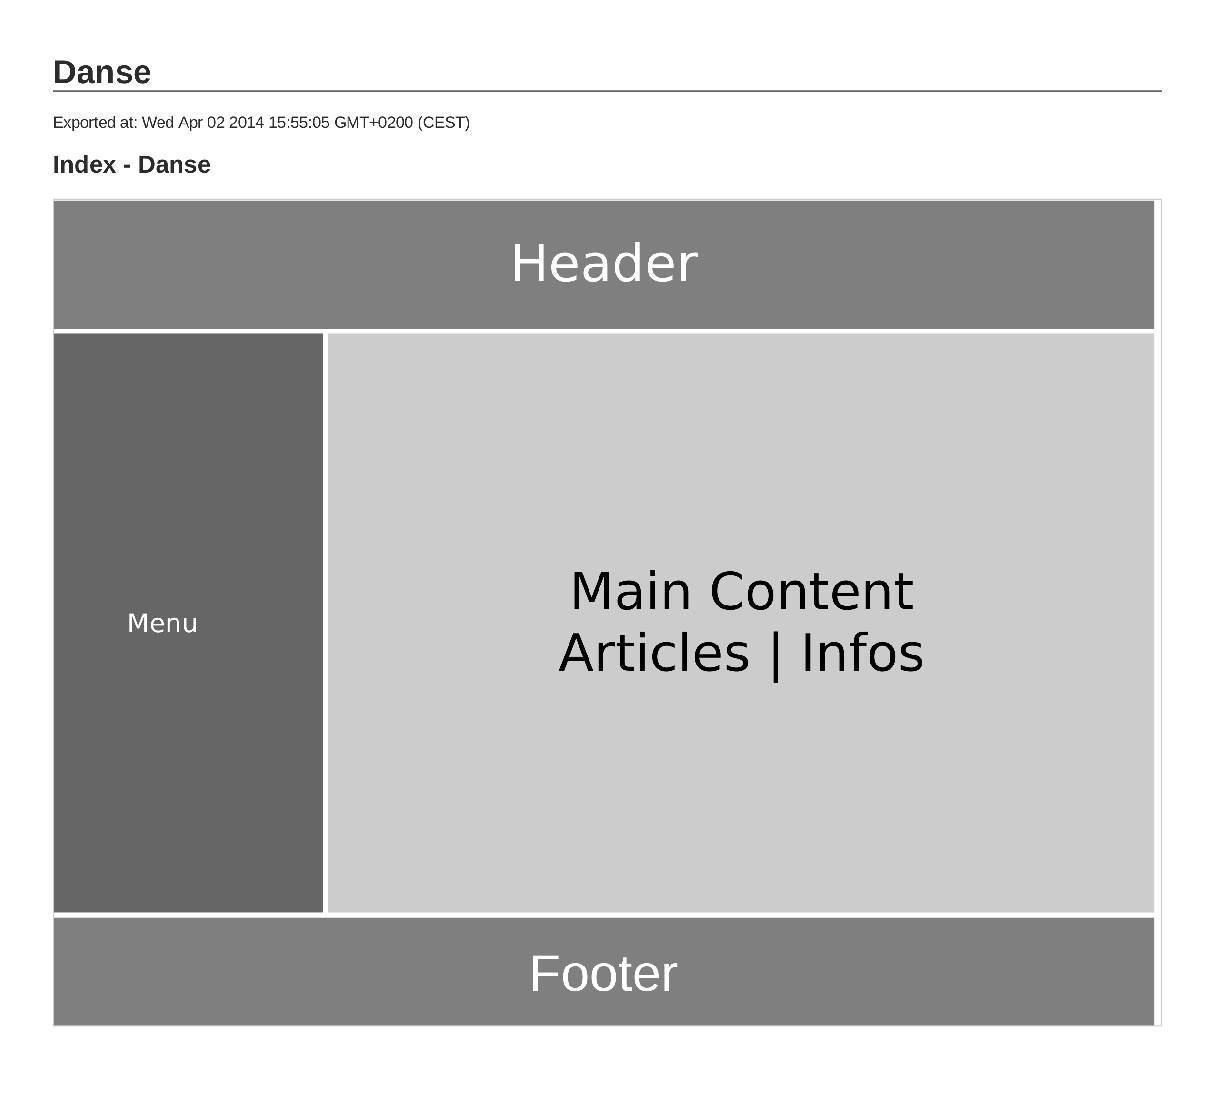
\includegraphics[height=10cm]{Zone-Danse.eps}
					\caption{Exemple de Zoning pour le site "Danse"}
					\label{fig:Zoning Danse}
				\end{figure}

			\paragraph*{Wireframe}J'ai ensuite préparé des Wireframes pour présenter les différentes possibilités offertes lors de la réalisation des sites. À ce moment là, le périmètre de l'application n'avais pas encore été défini, j'ai donc utilisé ces présentations pour expliquer les différents choix possible de réalisation.

				\begin{figure}[H]
					\centering
					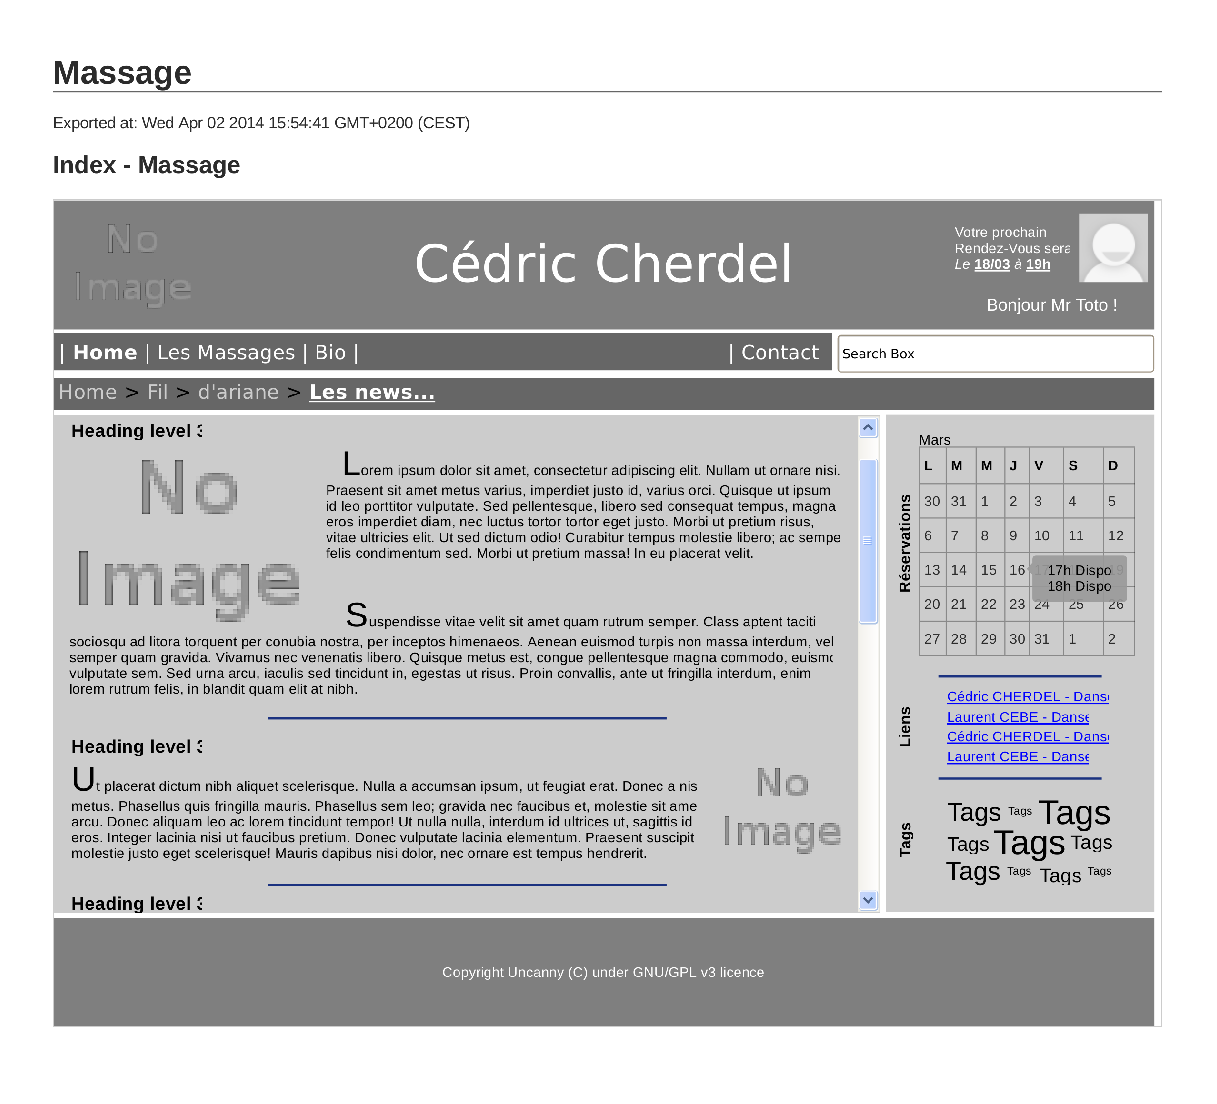
\includegraphics[height=10cm]{Wireframe-Massage_1.eps}
					\caption{Exemple de Wireframe pour le site "Massage"}
					\label{fig:Wireframe Massage}
				\end{figure}
				\begin{figure}[H]
					\centering
					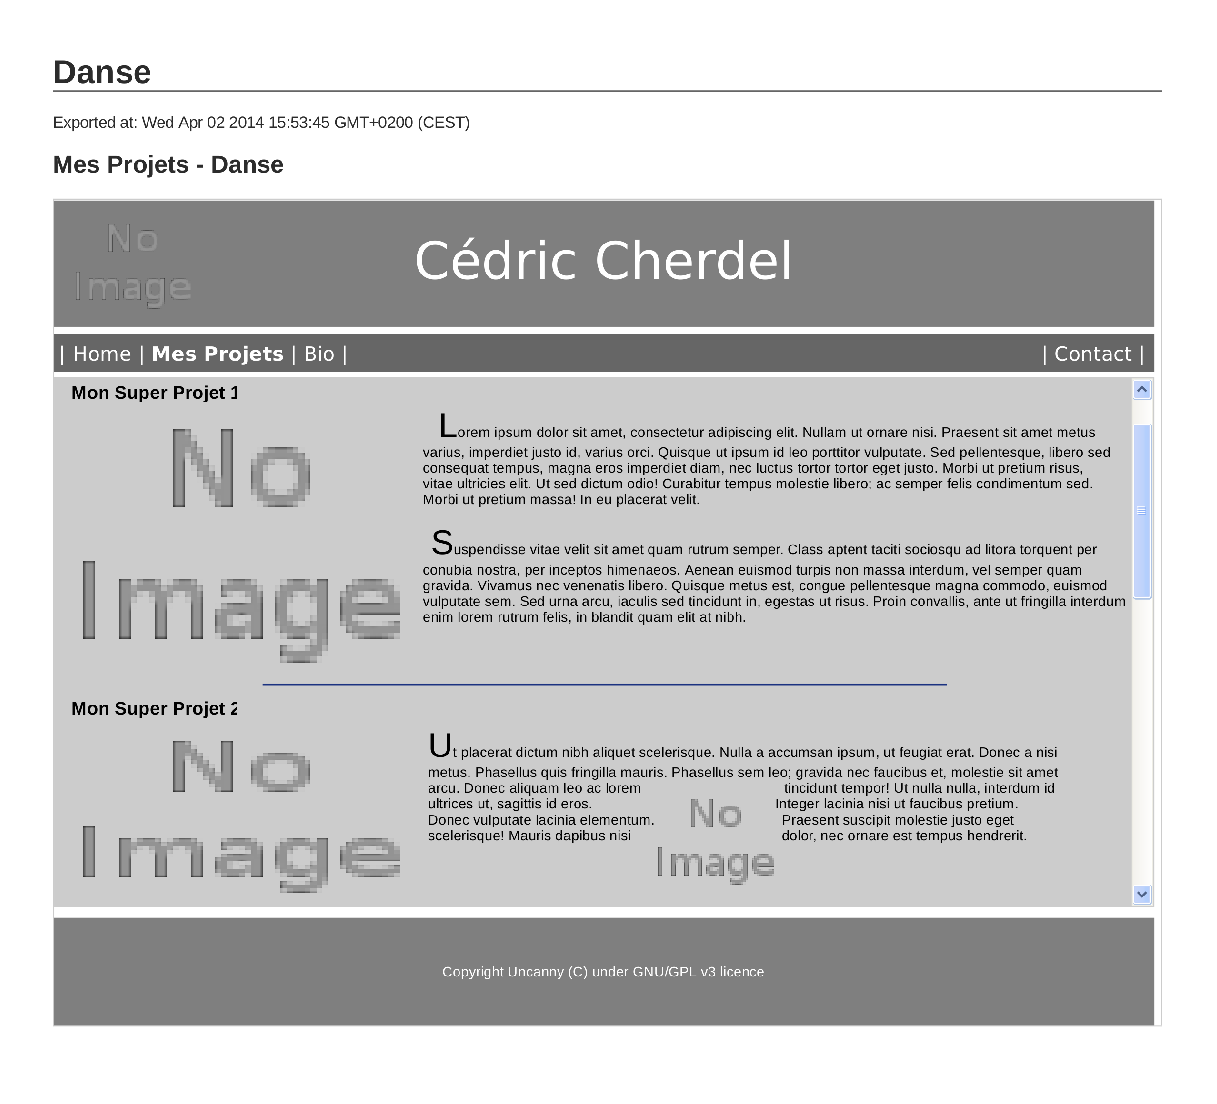
\includegraphics[height=10cm]{Wireframe-Danse_1.eps}
					\caption{Exemple de Wireframe pour le site "Danse"}
					\label{fig:Wireframe Danse}
				\end{figure}

			\paragraph*{Prototype}J'ai ensuite réalisé un prototype avec Wordpress pour présenter les différents développements requis avec Wordpress, et les contraintes liée à ce CMS. Ce prototype m'as permis de mettre en place sur un serveur de test Wordpress, MySQL ainsi que PHP5. J'en ai profité pour commencer à développer le thème des site pour Wordpress.

				\begin{figure}[H]
					\centering
					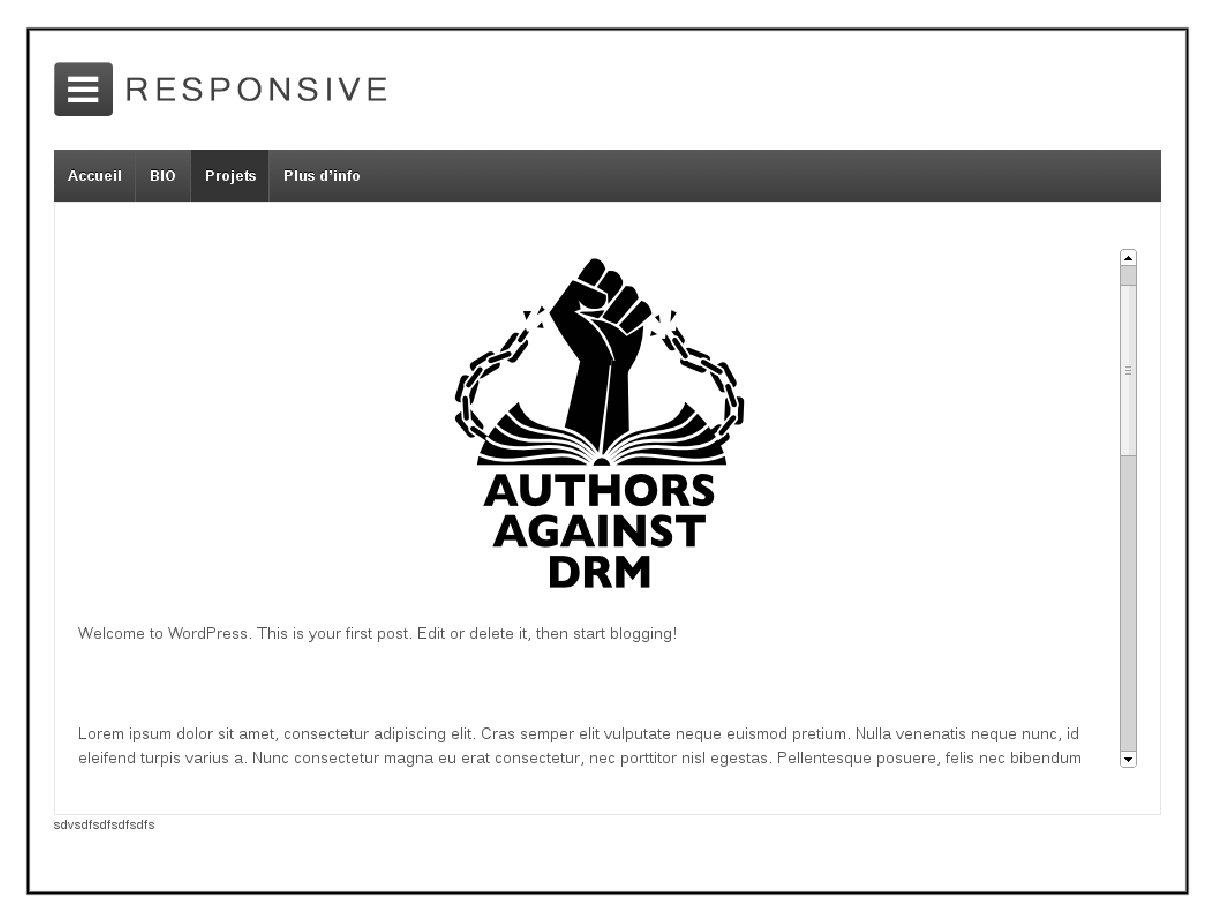
\includegraphics[height=10cm]{Prototype.eps}
					\caption{Prototype présenté pour validation}
					\label{fig:Prototype}
				\end{figure}

			\paragraph*{Styles Tiles \& Mockup}De son coté, Laurent Cebe, à réaliser des mokups et à commencé a travailler sur les styles tiles et la charte graphique.

				\begin{figure}[H]
					\centering
					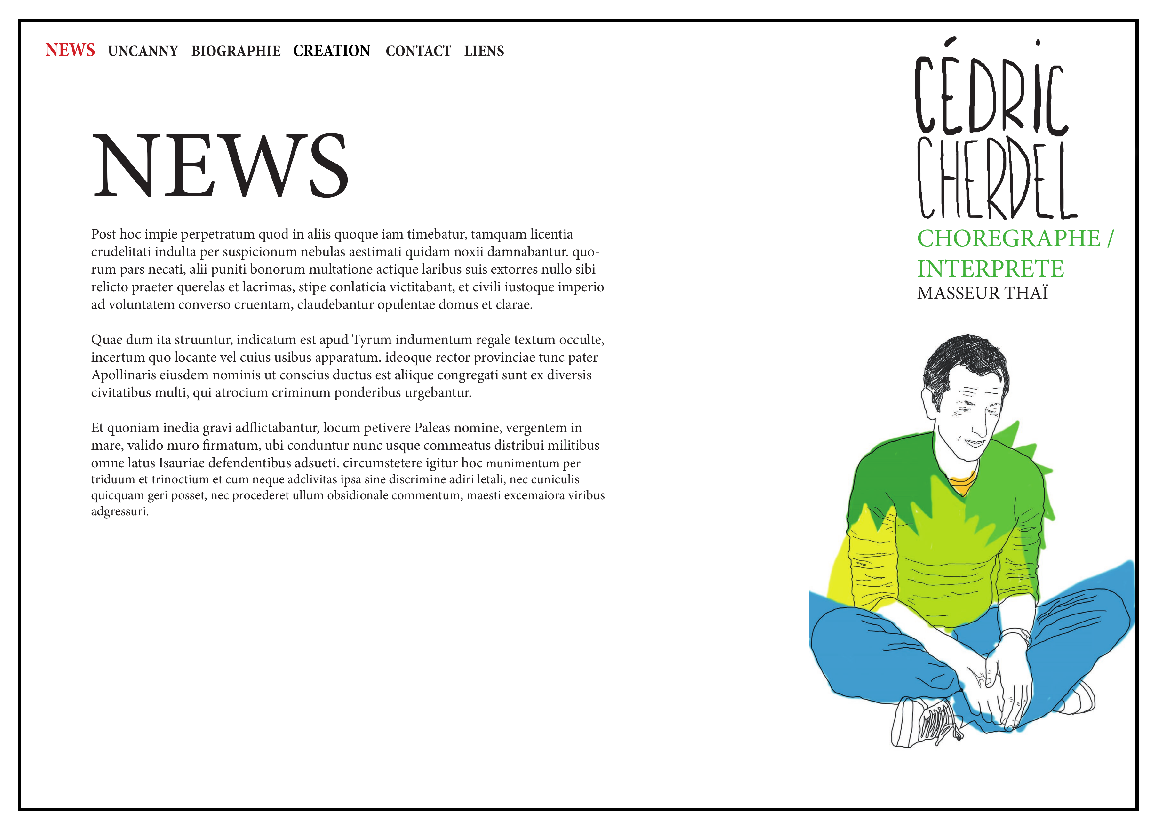
\includegraphics[height=10cm]{Mockup-Danse_1.eps}
					\caption{Mockup page d'accueil du site "Danse"}
					\label{fig:Mockup Danse}
				\end{figure}
				\begin{figure}[H]
					\centering
					
\includegraphics[height=10cm]{Mockup-Danse_2.eps}
					\caption{Mockup page projets du site "Danse"}
					\label{fig:Mockup Danse}
				\end{figure}\newpage

	\section{Planning: méthodes et outils}
		\subsection{Cahier des charges}
			\paragraph*{}J'ai commencé par rédiger un premier cahier des charge vierge (basé sur un modèle fournie par l'I.M.I.E.). Lors du premier jours, j'ai expliqué rapidement l'utilité d'un cahier des charge, puis dans une deuxièmes réunion, nous avons échangés autour des questions destiné à remplir ce cahier des charge. Enfin, lors de la réunion de validation, nous avons repris tout les points afin de les valider. Vous le trouverez en annexe 6.
		\subsection{Pert \& Gantt}
			\paragraph*{Prévisionnel}Les Pert et Gantt sont réalisé avec Planner\footnote{http://live.gnome.org/Planner : application Gnome en GNU/GPL v2}.
			\paragraph*{}J'ai commencé par ajouter les actions ainsi que les jalons dans Planner et j'ai estimé la charge de travail. Lors de ce projet, j'ai utilisé deux versions de mon Gantt, un Gantt prévisionnel (réalisé en début de projet) et un Gantt réel (avec une mise à jours des dates de validations en fonction des vrais date de rendez-vous)

				\begin{figure}[H]
					\centering
					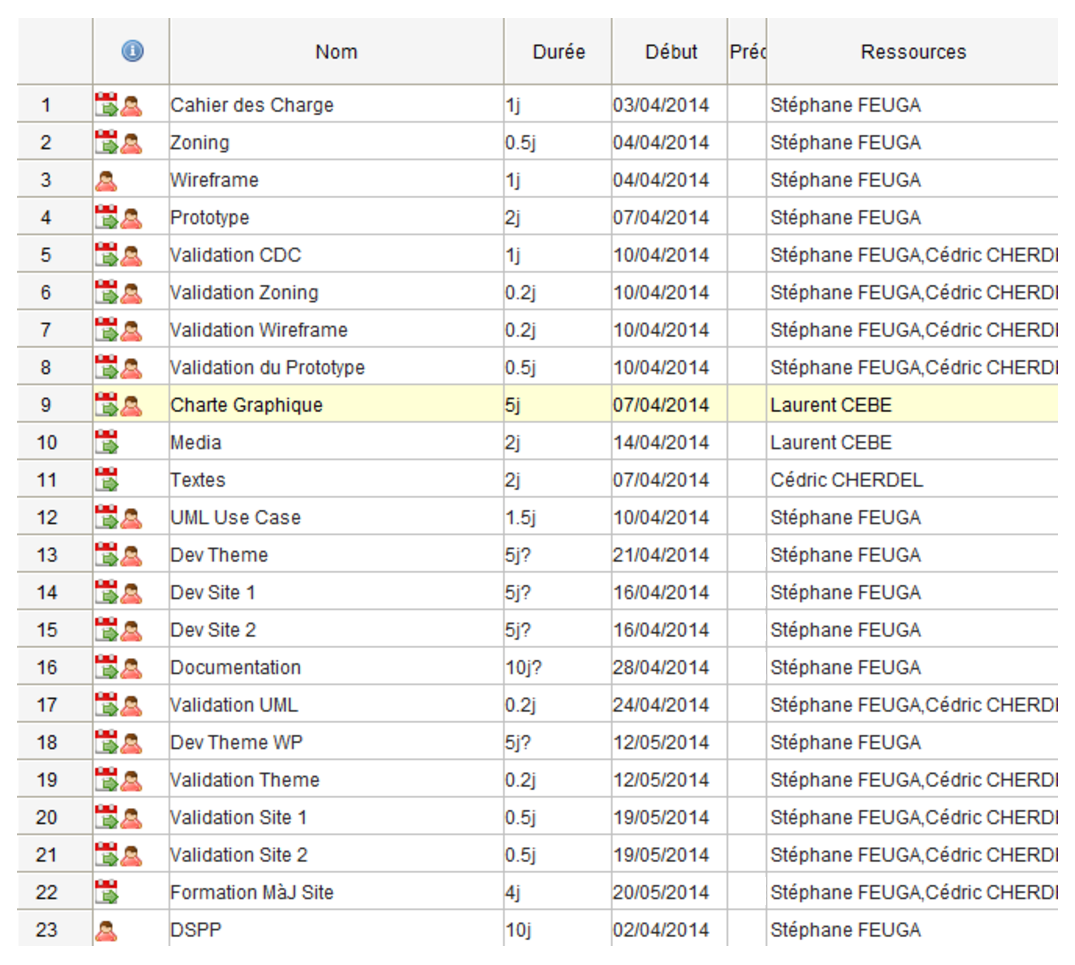
\includegraphics[height=10cm]{Gantt_Previsionnel_1.eps}
					\caption{Liste des actions et des Jalons}
					\label{fig:List des Actions Gantt Previsionnel}
				\end{figure}\newpage
			\paragraph*{}Puis j'ai lié les éléments avec leurs prédécesseurs, ce qui donne le graphique suivant: 

				\begin{figure}[H]
					\centering
					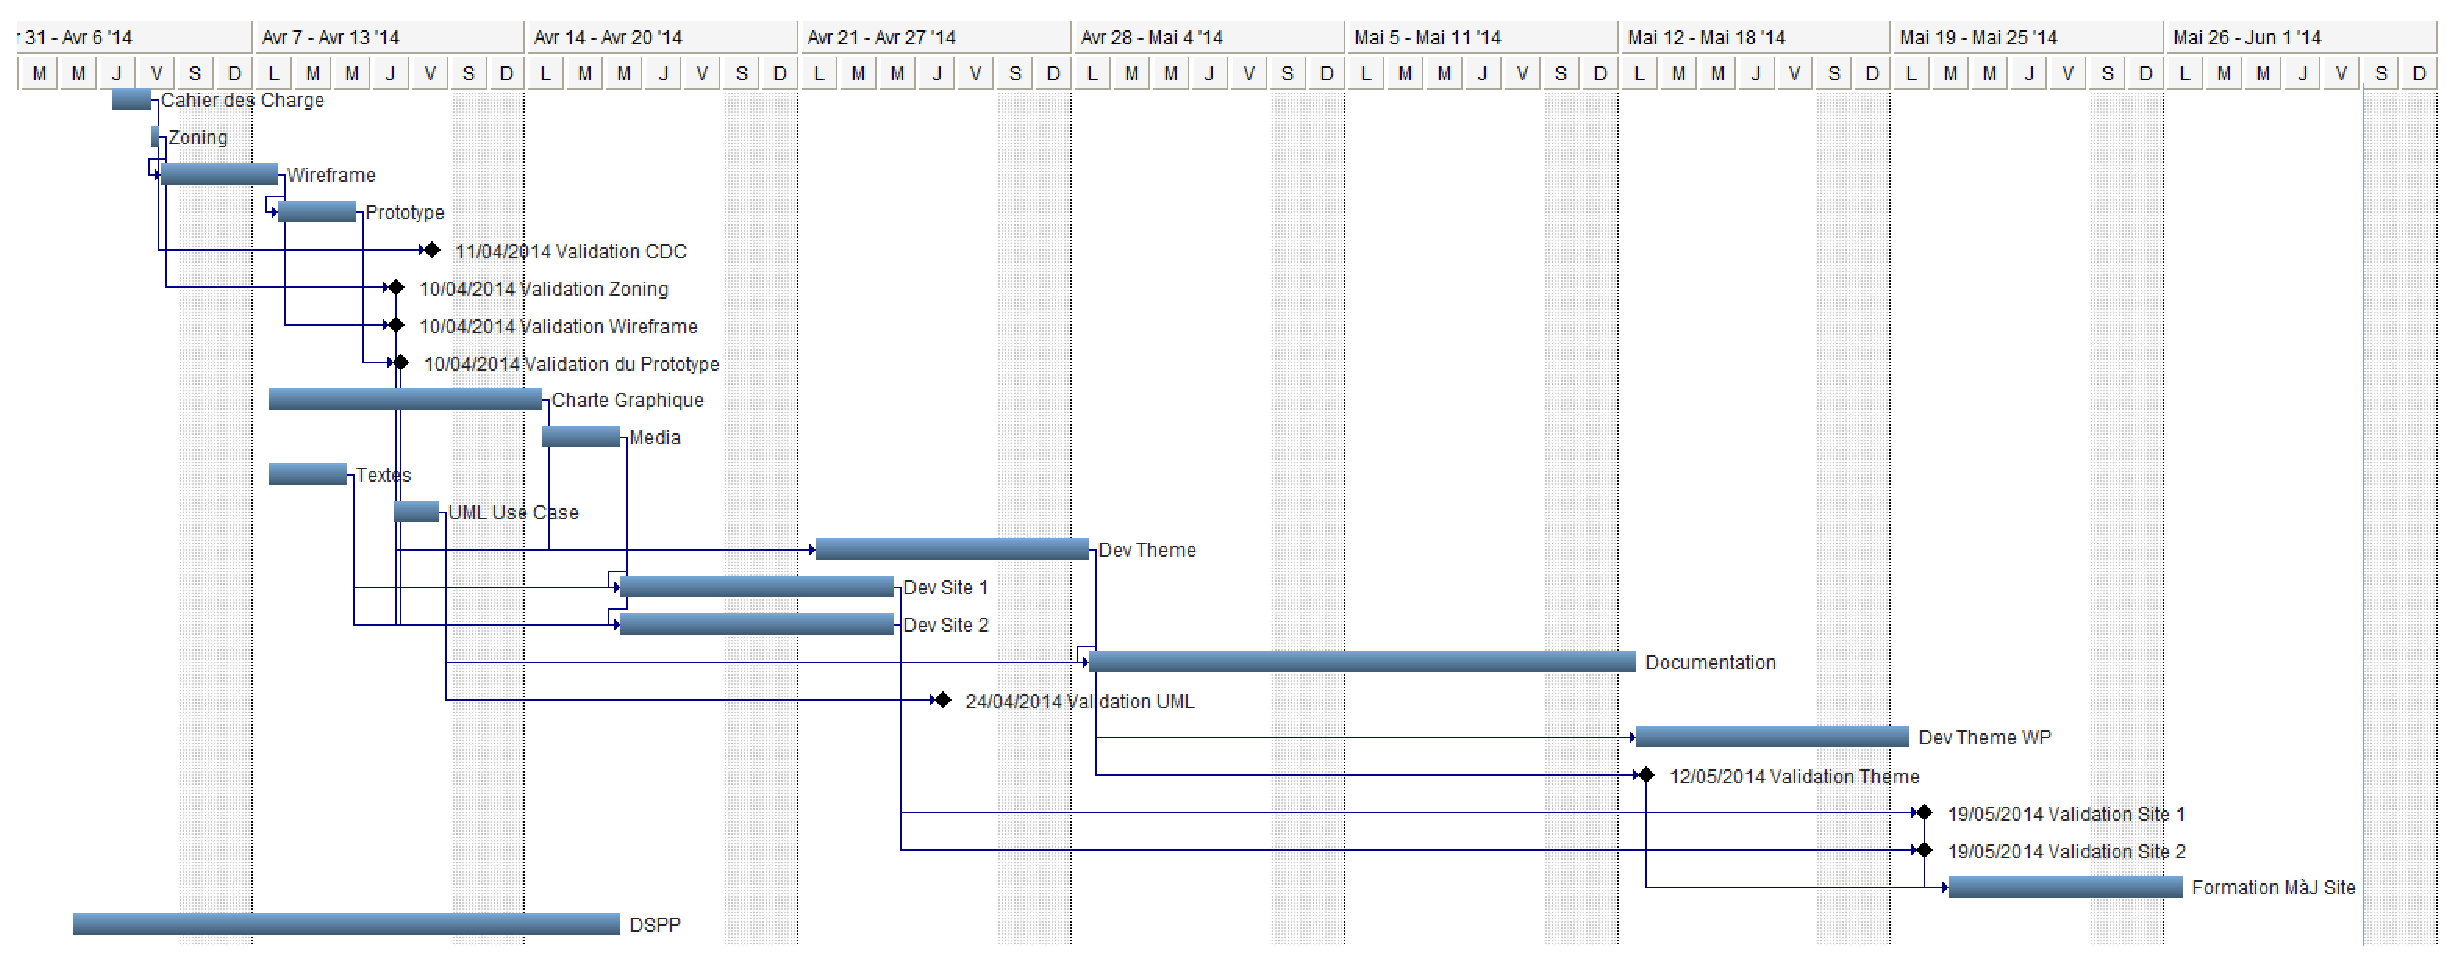
\includegraphics[width=\textwidth]{Gantt_Previsionnel_2.eps}
					\caption{Gantt prévisionnel fini}
					\label{fig:Graphique Gantt Previsionnel}
				\end{figure}
			\paragraph*{Réel}Enfin, j'ai dupliqué ce Gantt et je l'ai modifié en fonction des dates de validations réels. Ce qui donne le graphique suivant: 

				\begin{figure}[H]
					\centering
					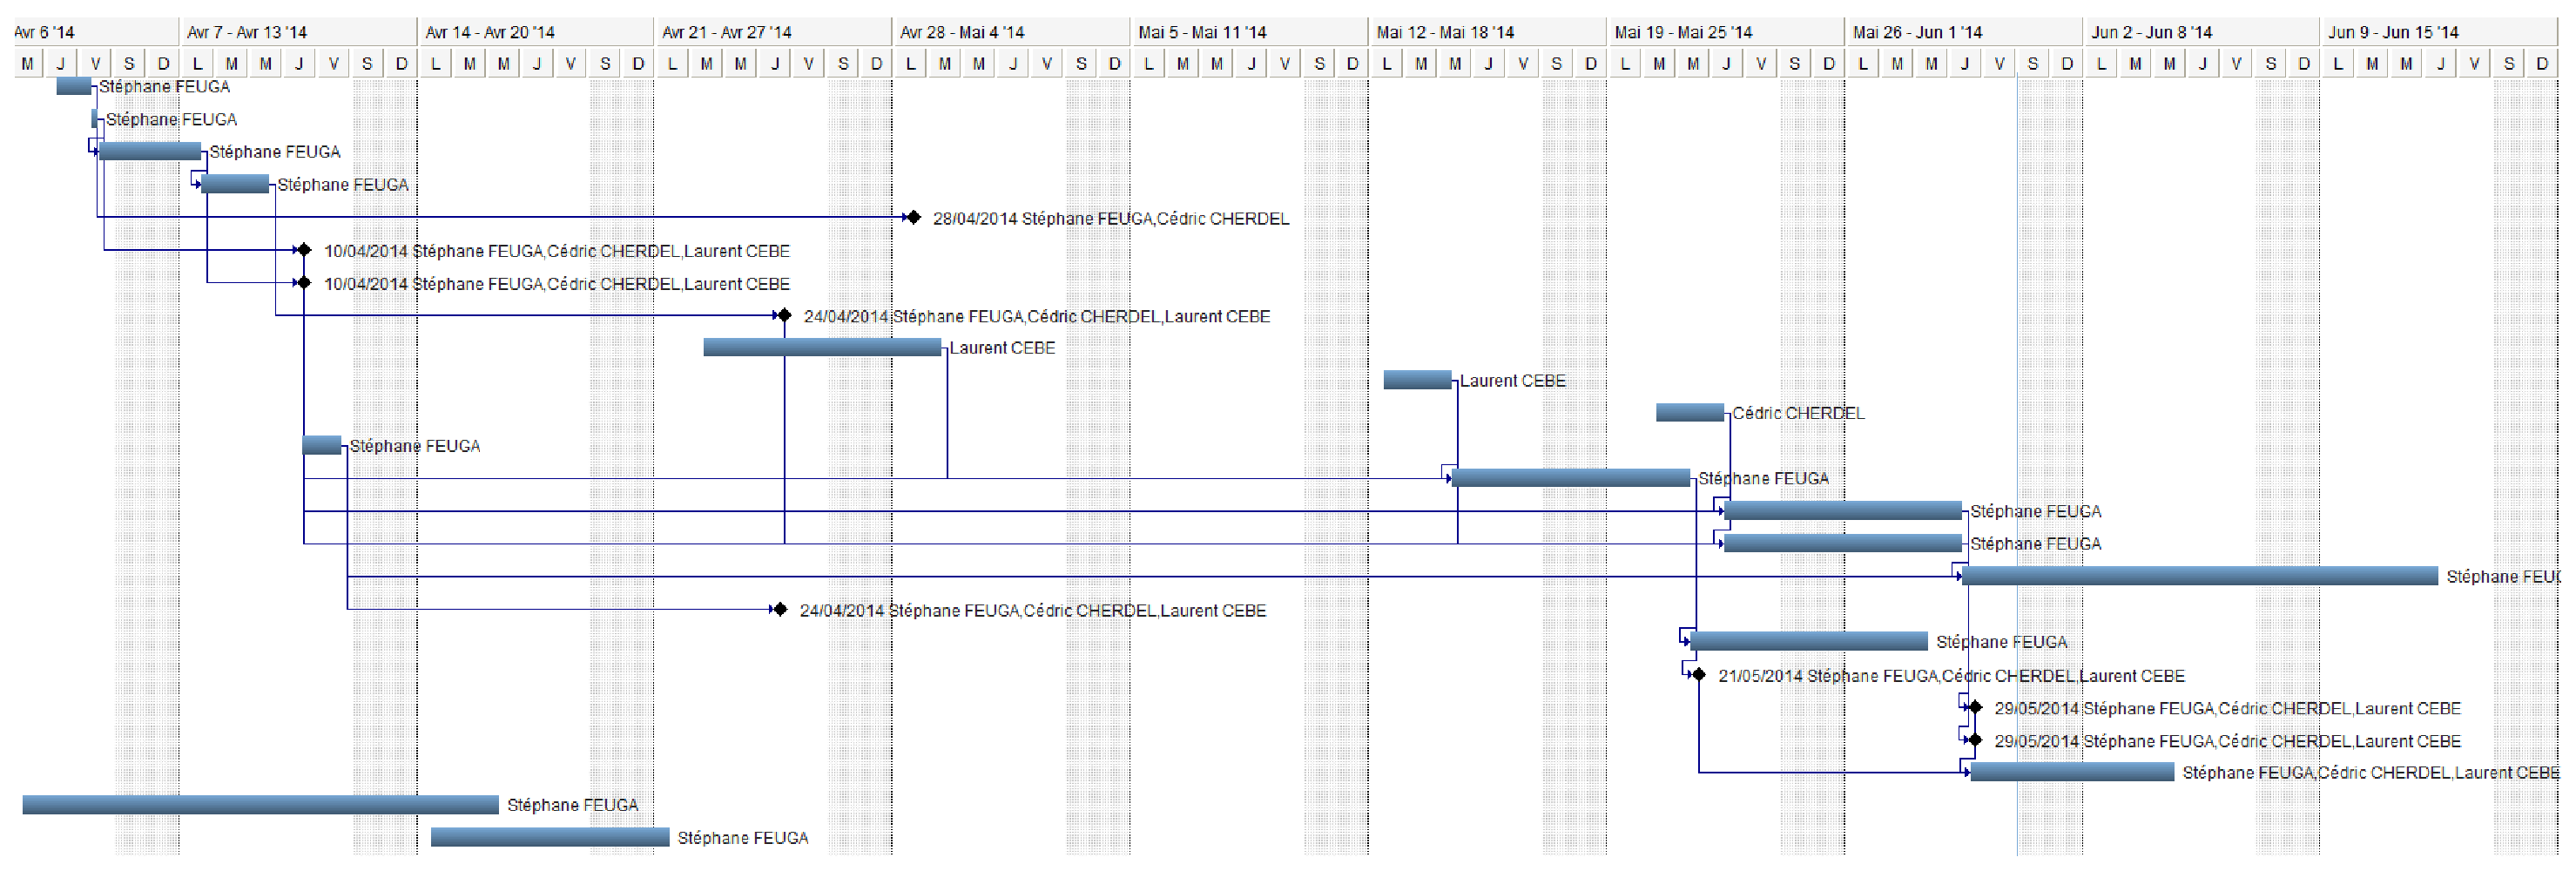
\includegraphics[width=\textwidth]{Gantt_Reel_2.eps}
					\caption{Gantt prévisionnel fini}
					\label{fig:Gantt Reel}
				\end{figure}
				\subparagraph*{}Les principaux problèmes de planning rencontré lors de ce stage sont lié au manque de disponibilité de Cédric et Laurent. Pendant cette période, ils se sont attelé à mettre en scène un nouveau spectacle qui sera présenté les 25 et 26 Juin prochains. J'ai du mettre certaines action en \textit{"pause"} le temps d'avoir les réponses et validations attendu. J'ai mis ce temps de \textit{"disponibilité"} à profits en me formant aux bases de Ruby pour JekyllRB. J'ai aussi eu du temps pour me documenté sur la danse contemporaine et sur les différentes techniques de massage Thaï.
				\newpage
		\subsection{Agilité, Scrum Board \& Git}
			\paragraph*{}Nous avons choisi de travailler en Agilité. Les Sprints sont d'une semaine et ne se rapport qu'à une fonctionnalité. Nous utilisons intensivement un Scrum Board\footnote{http://tsu3d.hestia.feralhosting.com/scrum}.
			\paragraph*{}Ce mode de fonctionnement m'as permis d'avoir un grande réactivité lors de changement important et l'utilisation d'un Scrum Board à permis à toutes les parties prenantes de suivre l'avancement du projet au jour le jour.
			Le Scrum board est réalisé en PHP, jQuery et HTML5. La base de donnée est en SQLite. C'est un fork réalisé depuis le projet kanboard\footnote{https://github.com/fguillot/kanboard}.
			\begin{figure}[H]
				\centering
				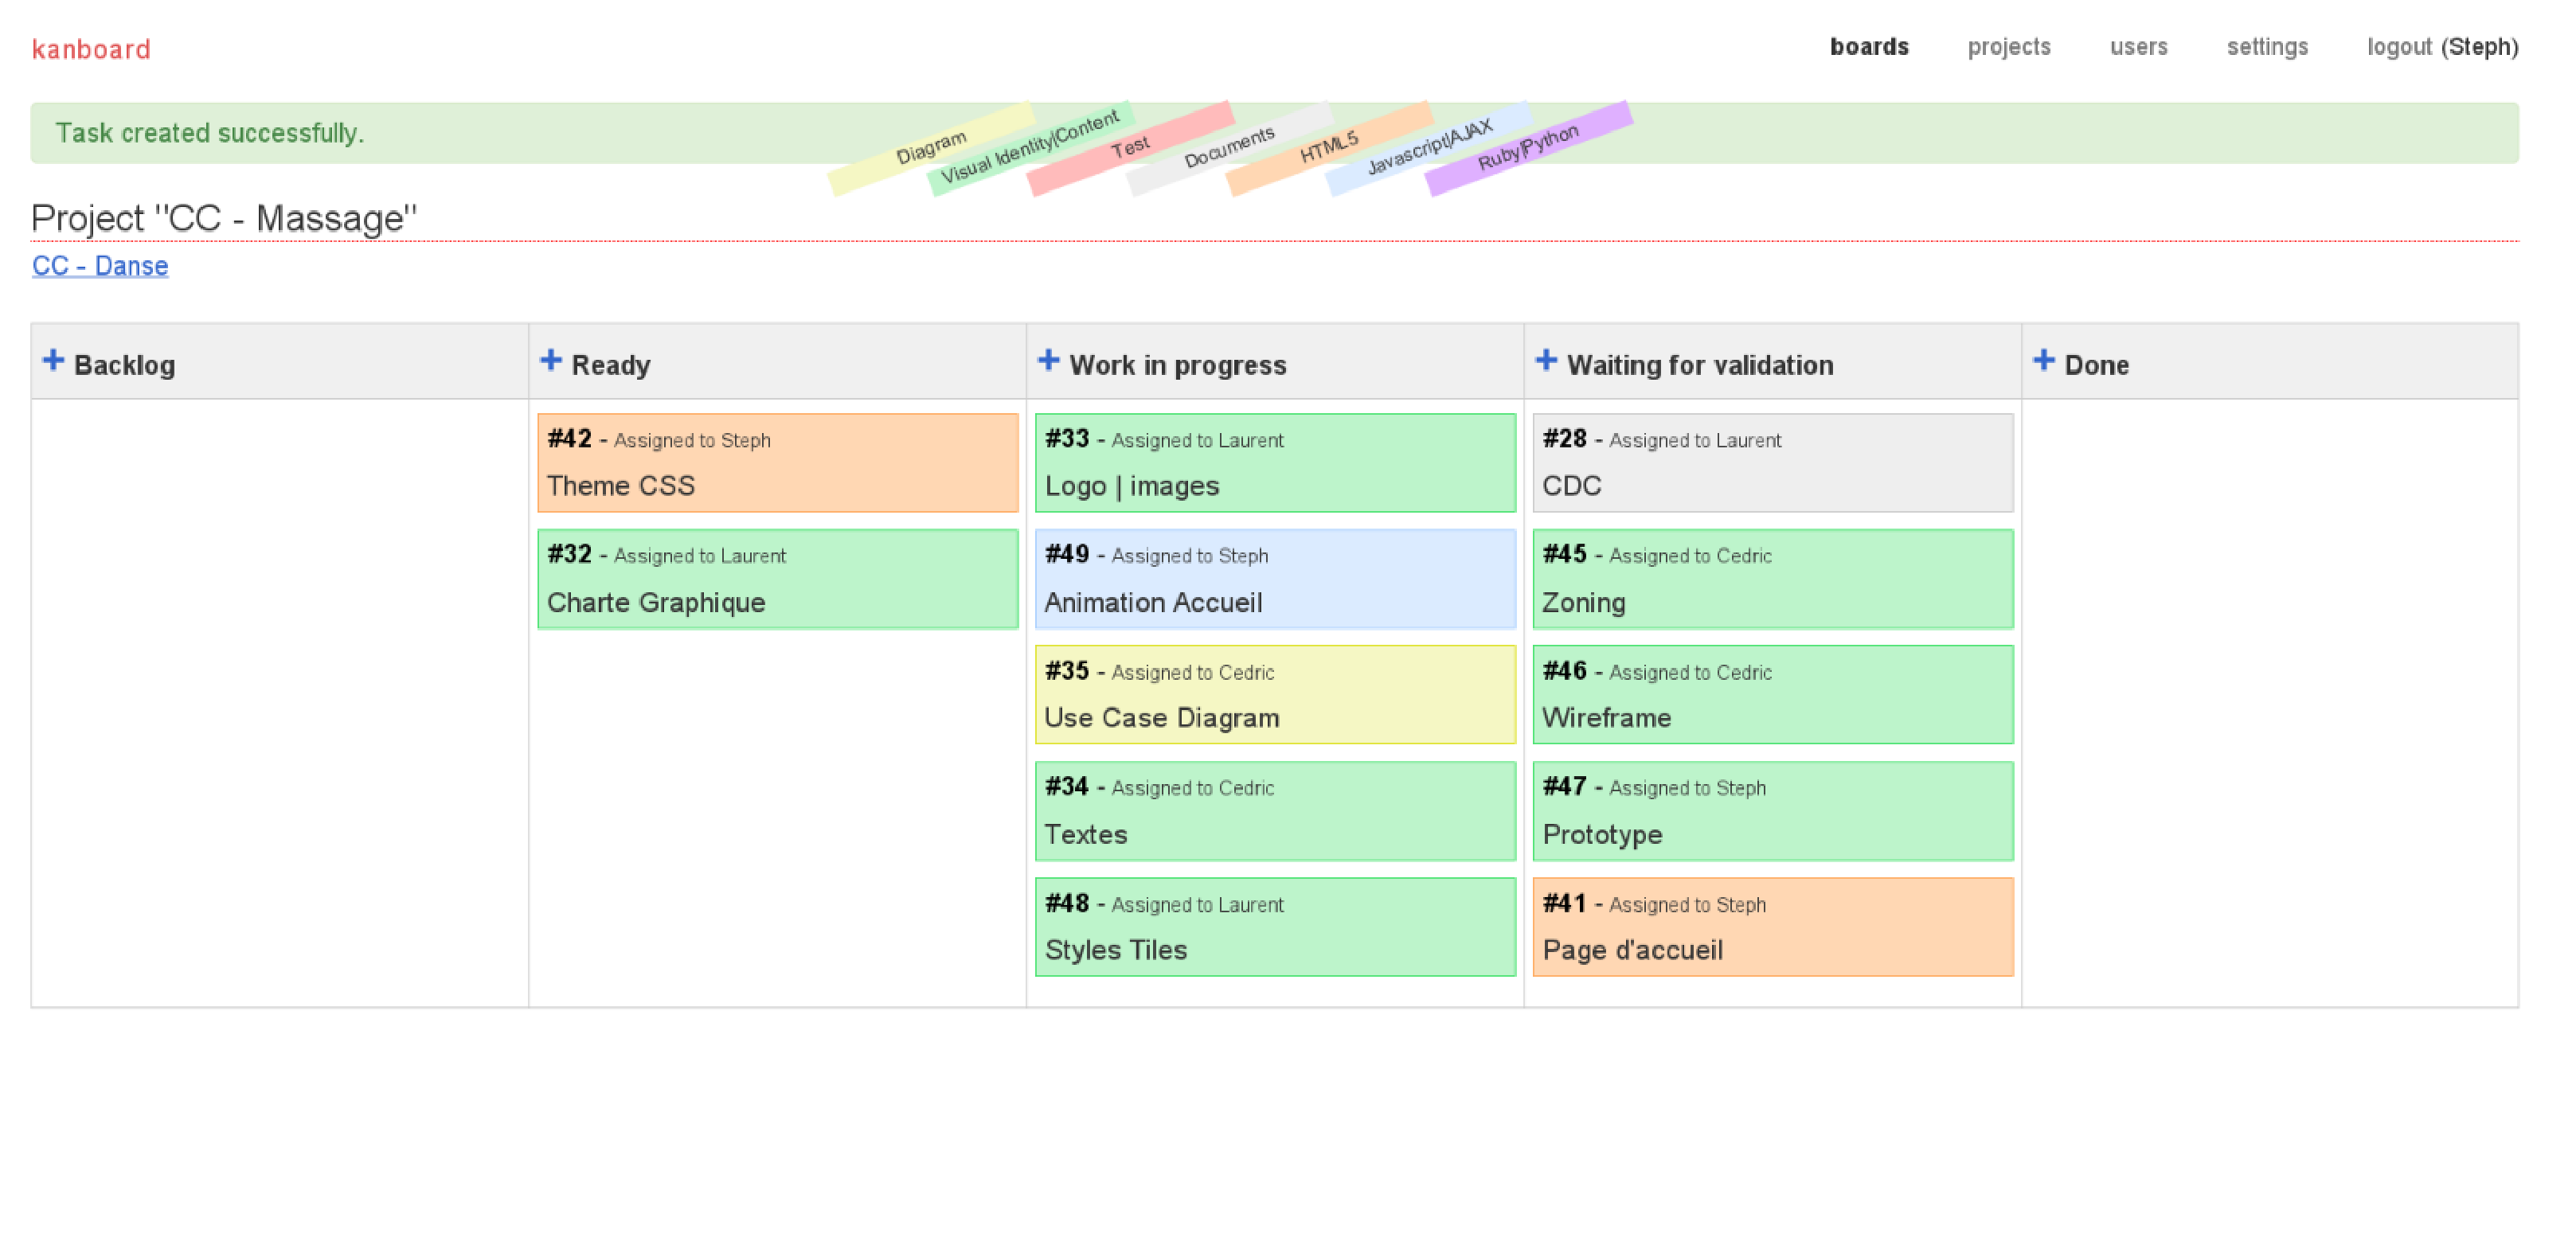
\includegraphics[width=\textwidth]{kanban1.eps}
				\caption[Kanban Board]{Exemple d'utilisation du Scrum Board pour le site "Massage"}
				\label{fig:Kanban Board}
			\end{figure}
			\begin{figure}[H]
				\centering
				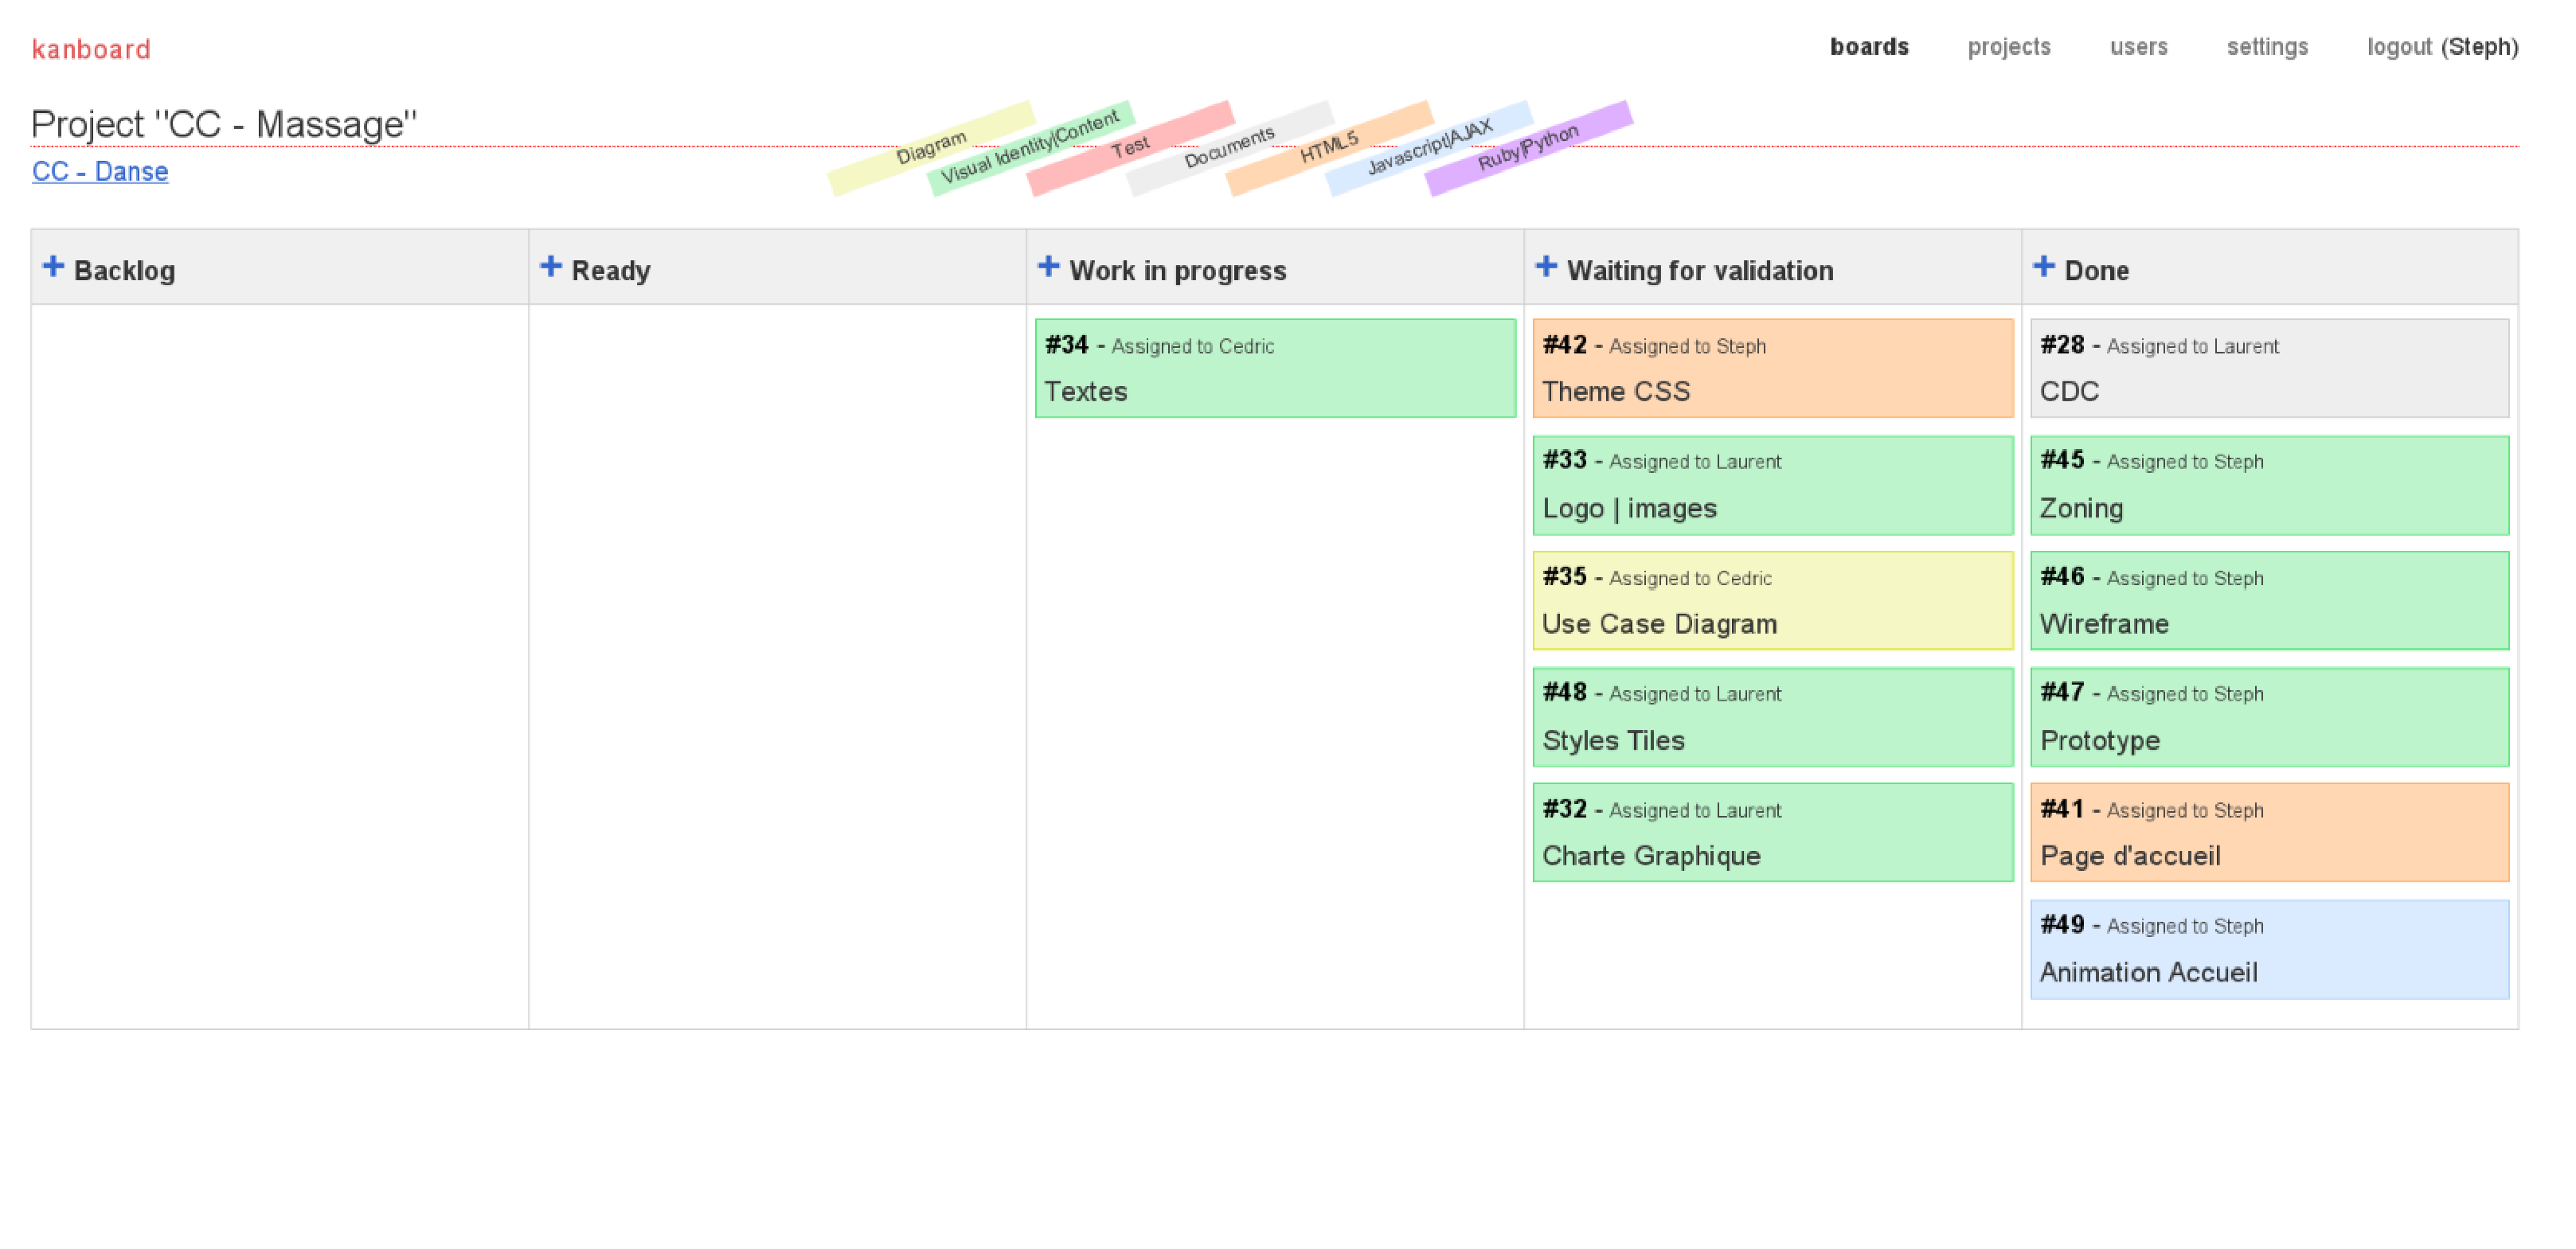
\includegraphics[width=\textwidth]{kanban2.eps}
				\caption[Kanban Board]{Scrum Board du site "Massage" Mis à Jour}
				\label{fig:Kanban Board v2}
			\end{figure}
			\paragraph*{}Le choix du gestionnaire de version à été rapide, j'utilise depuis fin 2005 GIT. Nous avons aussi choisi Gitorious comme plateforme d'hébergement car tout son code source est sous licence GNU/AGPL v3. L'utilisation de GIT\footnote{https://gitorious.org/uncanny} fut aussi intensive. Plusieurs \textit{"Repository"} ont été créé pour partager (et garder une trace des modifications) aussi bien les différents codes sources des sites, que les documentations, le cahier des charge (et ses annexes) ainsi que ce rapport. Ça a permis à tout le monde d'avoir accès à tout et de pouvoir suivre les modifications.\\
			Les différents répertoires sont:
				\begin{itemize}
					\item \textbf{theme}: Thème Wordpress (en cours de développement pour évolution futur).
					\item \textbf{site\_massage}: Site Massage sous Wordpress (en cours de développement pour évolution futur).
					\item \textbf{site\_danse}: Site Danse sous Wordpress (en cours de développement pour évolution futur).
					\item \textbf{site\_accueil}: Page d'accueil des deux sites (Réalisé en HTML5 et jQuery).
					\item \textbf{rapport\_de\_stage}: Ce rapport ainsi que toutes les annexes qui y sont liée.
					\item \textbf{cedriccherdel-massage}: Thème et Site réalisé avec JekyllRB.
					\item \textbf{cedriccherdel-danse}: Thème et Site réalisé avec JekyllRB.
				\end{itemize}
			\paragraph*{}À la suite de ce stage, il est prévu que je développe les fonctions manquantes à Wordpress pour ce projet. En effet, un des besoin exprimé au fil des rendez-vous à été une certaine \textit{automatisation"} de la création de contenu. La demande est la suivante: on créé un nouveau post et on ajoute dans le gestionnaire de média de Wordpress, les divers éléments liés à ce post. Ces éléments peuvent-être des pdf, des images et/ou des vidéos. Le but de cette automatisation est qu'en fonction des nom de fichiers et des nom de dossiers les contenant, tout les média présent pour ce projets sont automatiquement ajouté. Il n'est donc plus nécessaire de perdre du temps en "clic/sélection/clic" pour ajouter ces éléments dans le post.
\chapter{Conception}
	\section{Modélisations UML}
			\subsection{Use Case}
				\paragraph*{}J'ai commencé la modélisation de ce projet en effectuant des Uses-cases qui ont servit de validation pour le périmètre du développement.
				\paragraph*{}Ces schémas sont assez simple, mais m'ont permis d'expliquer plus simplement les fonctionnalités demandés. Une première version, avec des fonctionnalités n'apparaissant pas sur ces schémas, contenait une authentification des utilisateurs su site massage, un système de réservation de rendez-vous en ligne, la création et l'édition de newsletter depuis les sites via un back-office prévu à cette effet.
				\paragraph*{}Lors d'une séance de brainstorming, il est apparu que la prise de rendez-vous par les clients n'était pas souhaitable car ça impliquais de maintenir un calendrier de disponibilité à jours, ce qui n'est pas le cas actuellement. Pour ce qui est de la réalisation de newsletter, nous avons mis en place des modèles d'email réutilisable utilisant la charte graphique, ce qui à permis de ne pas développer des outils inutiles.
				\paragraph*{}Nous avons donc choisi de réalisé des sites plus simple mais répondant mieux aux besoins.
				\begin{figure}[H]
					\centering
					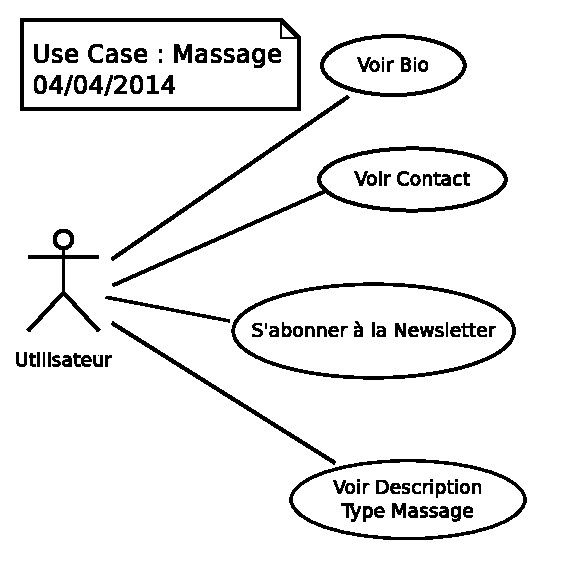
\includegraphics[height=10cm]{UseCase-Massage-User.eps}
					\caption[Use Case Utilisateur Massage]{Use Case d'un Utilisateur pour le site "Massage"}
					\label{fig:UseCase-Massage_User}
				\end{figure}
				\begin{figure}[H]
					\centering
					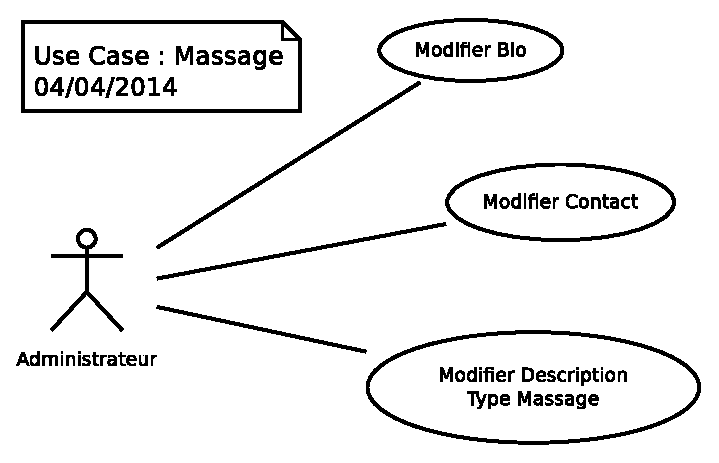
\includegraphics[height=10cm]{UseCase-Massage-Administrateur.eps}
					\caption[Use Case Administrateur Massage]{Use Case de l'administrateur pour le site "Massage"}
					\label{fig:UseCase-Massage_Admin}
				\end{figure}
				\begin{figure}[H]
					\centering
					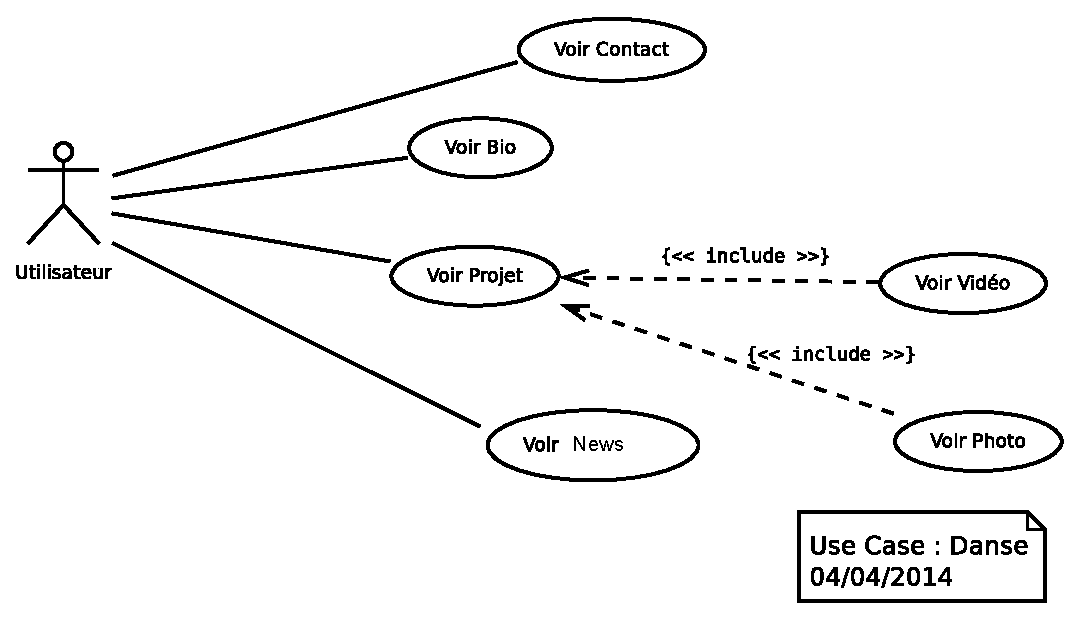
\includegraphics[height=10cm]{UseCase-Danse-User.eps}
					\caption[Use Case Utilisateur Danse]{Use Case d'un Utilisateur pour le site "Danse"}
					\label{fig:UseCase-Danse_User}
				\end{figure}
				\begin{figure}[H]
					\centering
					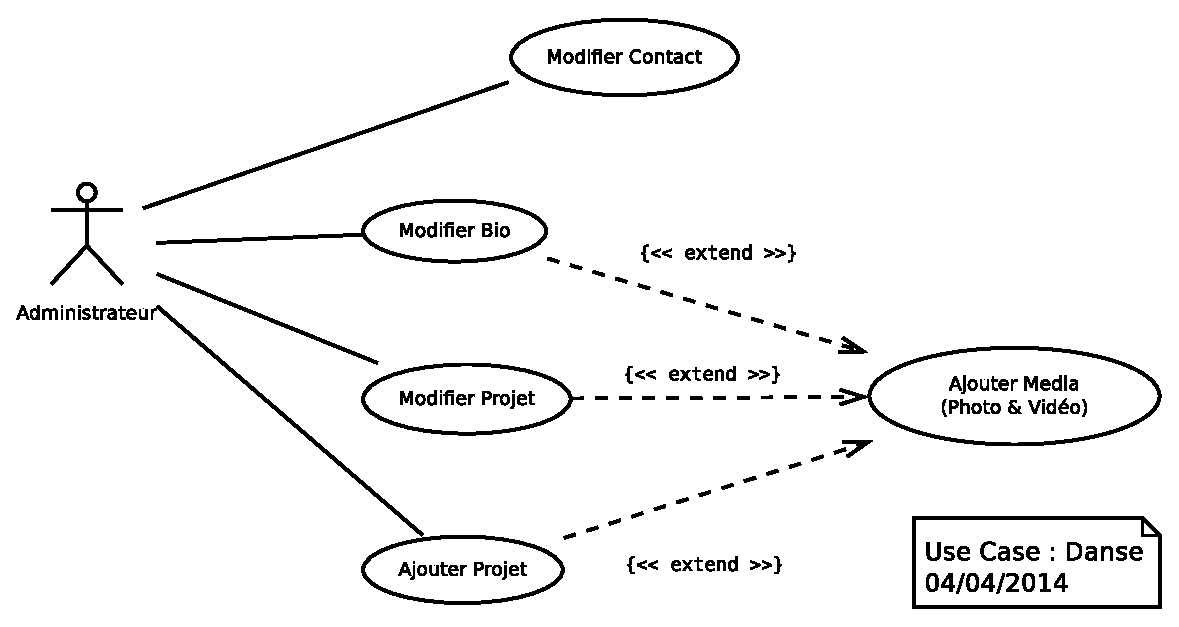
\includegraphics[height=10cm]{UseCase-Danse-Administrateur.eps}
					\caption[Use Case Administrateur Danse]{Use Case de l'administrateur pour le site "Danse"}
					\label{fig:UseCase-Danse_Admin}
				\end{figure}
				\newpage
				
	\section{Test \& Qualité}
		\subsection{Fonctionnel}
		\subsection{Intégration}

\chapter{Développement}
	\section{Technologies}
		\subsection{Page d'accueil}
			\paragraph{Pages HTML}
			\paragraph{CSS \& Responsive Design}
		\subsection{Thème}
			\paragraph{php}
			\paragraph{CSS \& Responsive Design}

\chapter{Déploiement \& Recette}
	\section{Prérequis techniques}
		\paragraph{}Un serveur web avec PHP 5.2.4 ou plus, MySQL 5.0 ou plus, le module Apache mod\_rewrite et un accès FTP.
	%\section{Scripts de mise en place de l'architecture logiciels}
	%\section{Scripts de déploiement de l'application}
	\section{Documentation:}
		\subsection{Développeur}Tout le code spécifique à été commenté. L'utilisation des documentations officiels de Wordpress\footnote{https://codex.wordpress.org}, de Less\footnote{http://lesscss.org}, de jQuery\footnote{http://api.jquery.com}, jQuery UI\footnote{http://api.jqueryui.com} ainsi que de php\footnote{http://www.php.net/manual/en/index.php} sont aussi vivement recommandé.
		\subsection{Administrateur}Une documentation sur l'administration générale et l'ajout de projet est disponible en annexe 7.
	\section{Recette}

\chapter{Bilan \& Conclusion}
	\paragraph*{}Ce stage m'as permis d'acquérir de nouvelles compétences aussi bien au niveau théorique que pratique. J'ai pu améliorer mes connaissances sur Wordpress et sur HTML5. Enfin, j'ai découvert le monde de la Danse contemporaine ainsi que les éléments nécessaires à la mise en place d'un spectacle.
	\paragraph*{}En effet, cette période de deux mois au sein de cette association m'a permis:
	\begin{itemize}
		\item De mieux connaitre le milieu associatif
		\item D'étendre mes connaissances acquises lors de la formation en réalisant un thème Wordpress en tenant compte des contraintes de mis en pages sur différentes plateformes
		\item D'utiliser les nouveautés d'animation en HTML5 pour la pages d'accueil
		\item De me familiariser avec les canvas HTML5 et plus généralement le SVG
		\item D'utiliser les librairies jQuery et jQuery UI
		\item D'avoir une meilleur vision des contraintes lié à un développement spécifique
	\end{itemize}
	\paragraph*{}La réalisation de ces tâches, l'aide de la communauté Wordpress France et l'implication des différents acteurs de ce stage, m'a permis d'atteindre les objectifs demandés, de devenir plus autonome et opérationnel dans le développement web, d'exploiter mes connaissances et d'en acquérir de nouvelles.
	\paragraph*{}Pour finir, je suis convaincu que cette expérience me permettra d'être en adéquation avec le marché de l'emploi dans la région.
	

%\chapter*{Lexique}

\chapter{Liste des Annexes}
	\begin{enumerate}
		\item CV
		\item Contenu pédagogique
		\item Présentation du titre
		\item RC
		\item REAC
		\item Cahier des Charges
		\item Documentation
	\end{enumerate}


\listoffigures \pagenumbering{Roman}
\listoftables

\end{document}
